% Options for packages loaded elsewhere
\PassOptionsToPackage{unicode}{hyperref}
\PassOptionsToPackage{hyphens}{url}
\PassOptionsToPackage{dvipsnames,svgnames,x11names}{xcolor}
%
\documentclass[
  letterpaper,
  DIV=11,
  numbers=noendperiod]{scrartcl}

\usepackage{amsmath,amssymb}
\usepackage{iftex}
\ifPDFTeX
  \usepackage[T1]{fontenc}
  \usepackage[utf8]{inputenc}
  \usepackage{textcomp} % provide euro and other symbols
\else % if luatex or xetex
  \usepackage{unicode-math}
  \defaultfontfeatures{Scale=MatchLowercase}
  \defaultfontfeatures[\rmfamily]{Ligatures=TeX,Scale=1}
\fi
\usepackage{lmodern}
\ifPDFTeX\else  
    % xetex/luatex font selection
\fi
% Use upquote if available, for straight quotes in verbatim environments
\IfFileExists{upquote.sty}{\usepackage{upquote}}{}
\IfFileExists{microtype.sty}{% use microtype if available
  \usepackage[]{microtype}
  \UseMicrotypeSet[protrusion]{basicmath} % disable protrusion for tt fonts
}{}
\makeatletter
\@ifundefined{KOMAClassName}{% if non-KOMA class
  \IfFileExists{parskip.sty}{%
    \usepackage{parskip}
  }{% else
    \setlength{\parindent}{0pt}
    \setlength{\parskip}{6pt plus 2pt minus 1pt}}
}{% if KOMA class
  \KOMAoptions{parskip=half}}
\makeatother
\usepackage{xcolor}
\setlength{\emergencystretch}{3em} % prevent overfull lines
\setcounter{secnumdepth}{-\maxdimen} % remove section numbering
% Make \paragraph and \subparagraph free-standing
\ifx\paragraph\undefined\else
  \let\oldparagraph\paragraph
  \renewcommand{\paragraph}[1]{\oldparagraph{#1}\mbox{}}
\fi
\ifx\subparagraph\undefined\else
  \let\oldsubparagraph\subparagraph
  \renewcommand{\subparagraph}[1]{\oldsubparagraph{#1}\mbox{}}
\fi


\providecommand{\tightlist}{%
  \setlength{\itemsep}{0pt}\setlength{\parskip}{0pt}}\usepackage{longtable,booktabs,array}
\usepackage{calc} % for calculating minipage widths
% Correct order of tables after \paragraph or \subparagraph
\usepackage{etoolbox}
\makeatletter
\patchcmd\longtable{\par}{\if@noskipsec\mbox{}\fi\par}{}{}
\makeatother
% Allow footnotes in longtable head/foot
\IfFileExists{footnotehyper.sty}{\usepackage{footnotehyper}}{\usepackage{footnote}}
\makesavenoteenv{longtable}
\usepackage{graphicx}
\makeatletter
\def\maxwidth{\ifdim\Gin@nat@width>\linewidth\linewidth\else\Gin@nat@width\fi}
\def\maxheight{\ifdim\Gin@nat@height>\textheight\textheight\else\Gin@nat@height\fi}
\makeatother
% Scale images if necessary, so that they will not overflow the page
% margins by default, and it is still possible to overwrite the defaults
% using explicit options in \includegraphics[width, height, ...]{}
\setkeys{Gin}{width=\maxwidth,height=\maxheight,keepaspectratio}
% Set default figure placement to htbp
\makeatletter
\def\fps@figure{htbp}
\makeatother

\KOMAoption{captions}{tableheading}
\makeatletter
\@ifpackageloaded{caption}{}{\usepackage{caption}}
\AtBeginDocument{%
\ifdefined\contentsname
  \renewcommand*\contentsname{Table of contents}
\else
  \newcommand\contentsname{Table of contents}
\fi
\ifdefined\listfigurename
  \renewcommand*\listfigurename{List of Figures}
\else
  \newcommand\listfigurename{List of Figures}
\fi
\ifdefined\listtablename
  \renewcommand*\listtablename{List of Tables}
\else
  \newcommand\listtablename{List of Tables}
\fi
\ifdefined\figurename
  \renewcommand*\figurename{Figure}
\else
  \newcommand\figurename{Figure}
\fi
\ifdefined\tablename
  \renewcommand*\tablename{Table}
\else
  \newcommand\tablename{Table}
\fi
}
\@ifpackageloaded{float}{}{\usepackage{float}}
\floatstyle{ruled}
\@ifundefined{c@chapter}{\newfloat{codelisting}{h}{lop}}{\newfloat{codelisting}{h}{lop}[chapter]}
\floatname{codelisting}{Listing}
\newcommand*\listoflistings{\listof{codelisting}{List of Listings}}
\makeatother
\makeatletter
\makeatother
\makeatletter
\@ifpackageloaded{caption}{}{\usepackage{caption}}
\@ifpackageloaded{subcaption}{}{\usepackage{subcaption}}
\makeatother
\ifLuaTeX
  \usepackage{selnolig}  % disable illegal ligatures
\fi
\usepackage{bookmark}

\IfFileExists{xurl.sty}{\usepackage{xurl}}{} % add URL line breaks if available
\urlstyle{same} % disable monospaced font for URLs
\hypersetup{
  pdftitle={Instructional Module},
  pdfauthor={Julie D. Halaman},
  colorlinks=true,
  linkcolor={blue},
  filecolor={Maroon},
  citecolor={Blue},
  urlcolor={Blue},
  pdfcreator={LaTeX via pandoc}}

\title{Instructional Module}
\author{Julie D. Halaman}
\date{}

\begin{document}
\maketitle

\subsection{Derivatives of Trigonometric
Functions}\label{derivatives-of-trigonometric-functions}

\subsubsection{Introduction}\label{introduction}

This module will briefly discuss Derivatives of Transcendental Functions
particularly Trigonometric Functions. The principles for Trigonometric
Functions rely heavily on the principles of Pythagorean Theorem. In the
right triangle \(\triangle ABC\) shown below,\(\angle BCA\) or simply
\(\angle C\) measures 90\(^{\circ}\) (hence making it a right triangle).
The legs of the triangle ABC are the line segments \emph{b} and
\emph{a}, the lines on either side of \(\angle C\), also called
\emph{legs.} Meanwhile, the \emph{hypotenuse} of the triangle is the
line segment \emph{c} which is opposite \(\angle C\).

\begin{center}
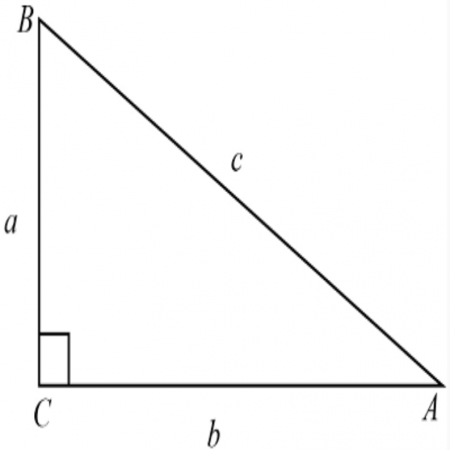
\includegraphics[width=1.86458in,height=\textheight]{IM-Halaman_files/mediabag/resize-1612330746441.png}
\end{center}

The Pythagorean theorem states that the sum of the squares of the
measures of the legs \emph{a} and \emph{b} of \(\triangle ABC\) is equal
to the square of the measure of the hypotenuse \emph{c} that is
\emph{a}\(^{2}\) + \emph{b}\(^{2}\) = \emph{c}\(^{2}\). By laying the
given right triangle \(\triangle ABC\) in a unit circle as shown below,
the formula \emph{a}\(^{2}\) + \emph{b}\(^{2}\) = \emph{c}\(^{2}\)
becomes \emph{a}\(^{2}\) + \emph{b}\(^{2}\) = 1. Recall that the radius
of a unit circle is equal to 1 unit, which in the triangle shown below,
corresponds to the hypotenuse \emph{c}.

Trigonometric functions, also known as Circular Functions, can be
defined as the functions of an angle of a triangle. Trig functions
identify the relationships between the angles and sides of a triangle.
The basic trigonometric functions are sine, cosine, tangent, cotangent,
secant and cosecant.

\subsubsection{The Trigonometric
Functions}\label{the-trigonometric-functions}

Solving for the values of the legs \emph{a} and \emph{b} of the triangle
above leads us to the use of the SOHCAHTOA formulas, which stemmed from
the three trigonometric functions sine (sin), cosine (cos), and tangent
(tan).

\subsubsection{The Sine Function}\label{the-sine-function}

The \emph{sine} of an angle is the ratio between the length of the
opposite side to the length of the hypotenuse. From the above diagram,
the value of the sine of \(\angle BAC\) will be:

\begin{itemize}
\tightlist
\item
  \textbf{Sin A =} \(\frac{Opposite}{Hypotenuse}\) = \(\frac{CB}{BA}\)
\end{itemize}

\subsubsection{The Cosine Function}\label{the-cosine-function}

The \emph{cosine} of an angle is the ratio of the length of the adjacent
side to the length of the hypotenuse. From the above diagram, the cos
function will be derived as follows:

\begin{itemize}
\tightlist
\item
  \textbf{Cos A =} \(\frac{Adjacent}{Hypotenuse}\) = \(\frac{CA}{BA}\)
\end{itemize}

\subsubsection{The Tangent Function}\label{the-tangent-function}

The \emph{tangent function} is the ratio of the length of the opposite
side to that of the adjacent side. From the diagram taken above, the tan
function will be the following:

\begin{itemize}
\tightlist
\item
  \textbf{Tan A =} \(\frac{Opposite}{Adjacent}\) = \(\frac{CB}{CA}\)
\end{itemize}

The tangent can also be expressed in terms of sin and cos as follows:

\begin{itemize}
\tightlist
\item
  \textbf{Tan A =} \(\frac{Sin A}{Cos A}\) = \(\frac{CB}{CA}\)
\end{itemize}

\subsubsection{Other Trigonometric
Formulas}\label{other-trigonometric-formulas}

Aside from the initial three functions, there are other trigonometric
formulas as shown in the following:

\begin{itemize}
\item
  \textbf{Sec A =} \(\frac{1}{Cos A}\) = \(\frac{Hypotenuse}{Adjacent}\)
  = \(\frac{BA}{CA}\)
\item
  \textbf{Cosec A =} \(\frac{1}{Sin A}\) =
  \(\frac{Hypotenuse}{Opposite}\) = \(\frac{BA}{CB}\)
\item
  \textbf{cot a =} \(\frac{1}{Tan A}\) = \(\frac{Adjacent}{Opposite}\) =
  \(\frac{CA}{CB}\)
\end{itemize}

Recall that sin\emph{x} and cos\emph{x} are defined and continuous
everywhere whereas the functions tan\emph{x}, sec\emph{x}, csc\emph{x},
and cot\emph{x} are continuous on their domains (all values of \emph{x}
where the denominator is non-zero).

Before we dive into the derivatives of trigonometric functions, let us
first discuss their limits.

Consider the unit circle given by the figure below.

\begin{center}
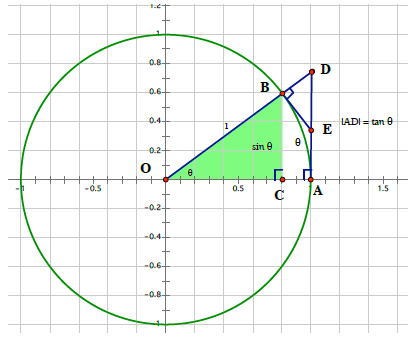
\includegraphics{clipboard-2032292710.png}
\end{center}

\subsubsection{Derivatives of Trigonometric
Functions}\label{derivatives-of-trigonometric-functions-1}

Now that we have reviewed trigonometric functions, we are now ready for
the derivation of trig functions.

For conformity, we will be using the Leibnitz Notation or Differential
Notation throughout this module.

The Leibnitz notation is given by: \[
\frac{df}{dx}
\]

or

\[
\frac{d}{dx}f(x) .
\]

Recall that \[
\frac{d}{dx}sin(x) = cos(x)
\]

and

\[
 \frac{d}{dx}cos(x)=-sin(x).
 \]

To remember which derivative contains the negative sign, recall the
graphs of the sine and cosine functions. At \emph{x=0}, \emph{sin(x)} is
increasing, and \emph{cos(x)} is positive, thus the derivative is a
positive \emph{cos(x)}. Meanwhile, just after \emph{x=0}, \emph{cos(x)}
is decreasing, and \emph{sin(x)} is positive, so the derivative must be
a negative \emph{sin(x)}.

Knowledge of the derivatives of sine and cosine allows us to find the
derivatives of all the other trigonometric functions using the quotient
rule.Recall the following identities:

\[tan(x)=\frac{sin(x)}{cos(x)}\] \[cot(x)=\frac{cos(x)}{sin(x)}\]
\[sec(x)=\frac{1}{cos(x)}\] \[csc(x)=\frac{1}{sin(x)}\]

Using the above knowledge, let us find the derivative of each function.

Example 1: Find the derivative of \(csc(x).\)

Recall that \(csc(x)=\frac{1}{sin(x)}.\)

Now let us apply the quotient rule.
\[\frac{d}{dx}csc(x)=\frac{sin(x)*0-1*cos(x)}{sin(x)^2}=-\frac{cos(x)}{sin(x)}*\frac{1}{sin(x)}=-cot(x)csc(x)\]

Example 2: Find the derivative of \(e^x*cos(x)+x^2.\)

Solution: To find this derivative, we will utilize the sum and product
rules.
\[\frac{d}{dx}(e^x*cos(x)+x^2)=e^x*cos(x)+e^x*(-sin(x))+2x=e^x(cos(x)-sin(x))+2x\]

The derivative of trigonometric functions can also be used to solve real
life problems. Consider the following problem and its solution.

Example 3: A police car is parked 40 feet from the road at the point
\emph{P} in the diagram below. Your vehicle is approaching on the road
as in the diagram below and the police are pointing a radar gun at your
car. Let \emph{x} denote the distance from your car to the police car
and let \(\theta\) be the angle between the line of sight of the radar
gun and the road. How fast is \emph{x} changing with respect to
\(\theta\) when \(\theta=\frac{\pi}{4}\)?

\begin{center}
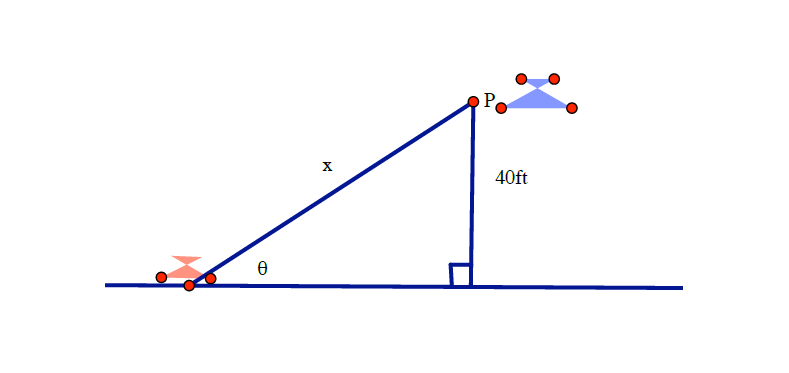
\includegraphics{images/Example 3 Image.png}
\end{center}

Solution: From the illustration, we can write:
\[\frac{40}{x}=sin(\theta).\]

Therefore, \[\frac{40}{sin(\theta)}=x\]

and \[\frac{dx}{d\theta}=40*\frac{-cos(\theta)}{sin^2(\theta)}.\]

When \(\theta=\frac{\pi}{4},\)

\(\frac{dx}{d\theta}=40*\frac{-cos(\frac{\pi}{4})}{sin^2(\frac{\pi}{4})}=40*\frac{-1/\sqrt2}{1/2}=-40\sqrt2\)
feet per radian.



\end{document}
